\documentclass[paper=screen,mathserif]{beamer}

\usetheme{CambridgeUS} 
\useinnertheme{circles}
\useoutertheme[footline=authortitle,subsection = false]{miniframes}
\setbeamercolor{palette tertiary}{fg=white, bg=white!42!black}
\setbeamercolor{alerted text}{fg=red!73!black}

%%%%%%
\usepackage{natbib}     % for references
\usepackage[osf]{sourcesanspro}
%\usepackage{sourcecodepro}
\usepackage{booktabs}
\usepackage{eulervm}
%\renewcommand{\ttdefault}{sourcecodepro}
\usepackage{import}
\usepackage{prodint}
\usepackage{bbm}
\usepackage{tabularx}
\usepackage{dcolumn}
\usepackage{color}
\usepackage{booktabs}
\usepackage{graphicx,rotating,epsfig,multirow,multicol,hhline}
\usepackage{amsmath,amsthm,amssymb,amsfonts}
\usepackage{listings}

\title[Literate Programming]{Introduction to Biostatistical Computing}
\subtitle{Literate Programming}

\author{Arthur Allignol}

\institute[]{\scriptsize{\url{arthur.allignol@uni-ulm.de}}}

\date{}
%%%%%%

\AtBeginSection[]
{
  \begin{frame}
    \frametitle{Table of Contents}
    \tableofcontents[currentsection]
  \end{frame}
}

\begin{document}

%%%%%% title page
\newcommand{\titlep}{yes}  % for titlepagelayout

{
\renewcommand{\insertframenumber}{}   % no page number on titlepage
\begin{frame}
\addtocounter{framenumber}{-1}
\titlepage
\end{frame}
}
%%%%%%

%\frame{\tableofcontents[currentsection]}

\section{Introduction}

\begin{frame}
  \frametitle{Introduction}
{\em An article about computational science in a scientific
  publication is not the scholarship itself, it is merely advertising
  of the scholarship. The actual scholarship is the complete software
  development environment and the complete set of instructions which
  generated the figures.}\\
--- D. Donoho

\begin{itemize}
\item The concept of reproducible research is based on the idea of
  {\em literate programming} such that the logic of the analysis is
  clearly represented in the final product by combining computer
  code/programs with ordinary human language

  $\Rightarrow$ Combine analysis code and report
\end{itemize}
\end{frame}

\begin{frame}{Literate Programming with R}
  2 main tools
  \begin{itemize}
  \item {\bf Sweave} (2002): a tool that allows to embed the R code for
    complete data analyses in latex documents. The purpose is to
    create dynamic reports, which can be updated automatically if data
    or analysis change.
    \begin{itemize}
    \item Sweave is part of every R installation
    \end{itemize}
  \item {\bf knitr}: ``The knitr package was designed to be a
    transparent engine for dynamic report generation with R, solve
    some long-standing problems in Sweave, and combine features in
    other add-on packages into one package''

    e.g., caching, html and markdown
  \end{itemize}
\end{frame}

\begin{frame}{Data Example}
  \framesubtitle{Televisions, Physicians, and Life Expectancy}
  The data set contains information on
  \begin{itemize}
  \item Life expectancies in 40 countries with population $\geq$ 20
    millions (1990)
    \begin{itemize}
    \item For female and male. Average used as the country's overall
      life expectancy
    \end{itemize}
  \item Number of people per television set 
  \item Number of people per physician 
  \end{itemize}
  Data set taken from the {\em The World Almanac and Book of Facts},
  1993
\end{frame}

\begin{frame}[fragile]{Data Example}
  \framesubtitle{Televisions, Physicians, and Life Expectancy}
\begin{verbatim}
     Country life    tv phys fem male
1  Argentina 70.5   4.0  370  74   67
2 Bangladesh 53.5 315.0 6166  53   54
3     Brazil 65.0   4.0  684  68   62
4     Canada 76.5   1.7  449  80   73
5      China 70.0   8.0  643  72   68
6   Colombia 71.0   5.6 1551  74   68
\end{verbatim}
\end{frame}

\begin{frame}{Data Example}
  \framesubtitle{Televisions, Physicians, and Life Expectancy}
  
  Is the number of people per TV set a good predictor of life expectancy?

\end{frame}

\section{Sweave}

\begin{frame}{Sweave}

  %{\bf A plot of the workflow} 
  \centering
  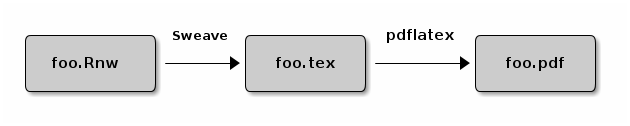
\includegraphics[width = \textwidth]{graphics/sweave_workflow.png}
  \begin{columns}[T]
    \begin{column}{.33\textwidth}
      \begin{itemize}
      \item A .tex file with .Rnw extension
      \item Include R code as 'chunks' or inline
      \end{itemize}
    \end{column}
    \begin{column}{.33\textwidth}
      \begin{itemize}
      \item .Rnw file converted to .tex using Sweave
      \item The .tex file contains output from R; no raw code
      \end{itemize}
    \end{column}
    \begin{column}{.33\textwidth}
      \begin{itemize}
      \item .tex file converted to .pdf (or .ps, .dvi) 
      \end{itemize}
    \end{column}
  \end{columns}
\end{frame}

\begin{frame}[fragile]{Sweave}
  
  {\scriptsize
    \begin{block}{.Rnw file}
\begin{verbatim}
\documentclass{article}
\usepackage{Sweave}

\begin{document}

Some R code:
<<>>=
x <- rnorm(1000)
@ 
Let's display an histogram of {\tt x}
\begin{figure}[!h]
  \centering
<<myhist, fig = TRUE, eps = FALSE>>=
hist(x)
@ 
\caption{An histogram of {\tt x}}
   \label{fig:hist}
\end{figure}

\end{document}
\end{verbatim}
    \end{block}}
  
\end{frame}

\begin{frame}[fragile]{Sweave}
  \begin{block}{.tex file}
{\tiny
\begin{verbatim}
\documentclass{article}
\usepackage{Sweave}

\begin{document}

Some R code:
\begin{Schunk}
\begin{Sinput}
> x <- rnorm(1000)
\end{Sinput}
\end{Schunk}

Let's display an histogram of {\tt x}
\begin{figure}[!h]
  \centering
\begin{Schunk}
\begin{Sinput}
> hist(x)
\end{Sinput}
\end{Schunk}
\includegraphics{simple_example-myhist}
\caption{An histogram of {\tt x}}
   \label{fig:hist}
\end{figure}

\end{document}
\end{verbatim}}
  \end{block}
\end{frame}

\begin{frame}{Sweave}
  \centering
  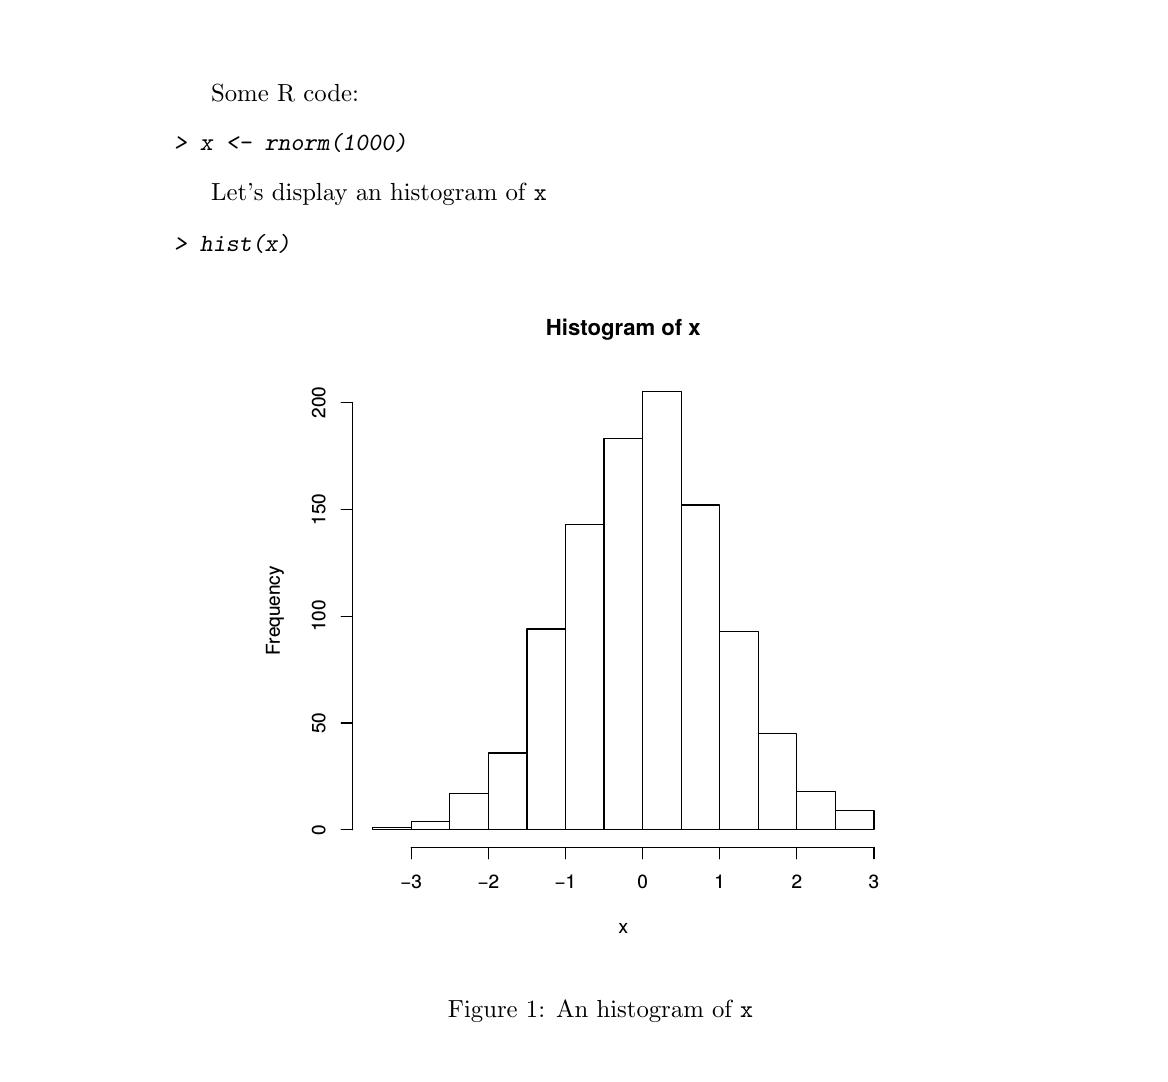
\includegraphics[width = .7\linewidth]{graphics/image_simple_rnw.jpeg}
\end{frame}

\begin{frame}[fragile]{Sweave}
  \framesubtitle{Code chunks}
  
  R code is entered in the \LaTeX$\;$document using {\em code chunks}.
  \begin{block}{}
\begin{verbatim}
<< >>=
@
\end{verbatim}
  \end{block}
  \begin{itemize}
  \item Text within the code chunk is interpreted as R code
  \item Arguments for the code chunk are entered within \verb=<<here>>==
  \end{itemize}
\end{frame}

\begin{frame}[fragile]{Sweave}
  \framesubtitle{Code chunks options}
  \begin{itemize}
  \item \verb=eval=: Default is \verb=TRUE=. If set to \verb=FALSE=,
    code is not evaluated
  \item \verb=echo=: Include R code in the output file. Default is \verb=TRUE=
  \item \verb=keep.source=: Default to \verb=FALSE=. If \verb=TRUE=,
    the original source code is copied to the file when
    echoing. Otherwise it gets through R's parsing engine
  \item \verb=results=: Default to \verb=verbatim=, the output of the
    R code is copied ``verbatim'' to the file. Other option is
    \verb=tex= for latex output, e.g., table, or \verb=hide= 
  \item \verb=include=: Default to \verb=TRUE=. If you want to place
    the figure yourself, add \verb=include==\verb=FALSE=
  \end{itemize}  
\end{frame}

\begin{frame}[fragile]{Sweave}
  \framesubtitle{Code chunks options}
  \begin{itemize}
  \item \verb=fig=: Default to \verb=FALSE=. Indicate whether the code
    chunk produces a graphical output
  \item \verb=eps=: Indicates whether a .eps figure should be
    generated. Default is \verb=TRUE= but ignored if \verb=fig= is
    \verb=FALSE=
  \item \verb=pdf=: generate .pdf figure. Default to \verb=TRUE=
  \item \verb=width= and \verb=height=: width and height of the
    figures in inches (default is 6)
  \end{itemize}
  \begin{block}{}
\begin{verbatim}
\SweaveOpts{option1 = value1, option2 = value2, ...} 
\end{verbatim}
  \end{block}
in the preamble sets default for all the code chunks in the document    
\end{frame}

\begin{frame}[fragile]{Sweave}
  \framesubtitle{Named code chunks}

  Named code chunks can be reused in other code chunks later in the
  document

  \begin{block}{}
\begin{verbatim}
<<a>>=
x <- 10
@
\end{verbatim}
  \end{block}

  \begin{block}{}
\begin{verbatim}
<<b>>=
x + y
@
\end{verbatim}
  \end{block}
  \begin{block}{}
\begin{verbatim}
<<c>>=
<<a>>
y <- 20
<<b>>
@
\end{verbatim}
  \end{block} 
\end{frame}

\begin{frame}[fragile]{Sweave}
  \framesubtitle{Figures}

  Easy to include figures in your document

  \begin{block}{}
\begin{verbatim}
\begin{figure}
\begin{center}
<<my_fig, fig=TRUE, echo=FALSE, width=10, eps = FALSE>>=
plot(x, y)
@
\caption{A beautiful figure}
\end{center}
\end{figure}
\end{verbatim}
  \end{block}
The chunk name is used as figure name, i.e., {\em myfile}-myfig.pdf
\end{frame}

\begin{frame}[fragile]{Sweave}
  \framesubtitle{Figures}
Alternative:
\begin{block}{}
\begin{verbatim}
<<my_fig, fig=TRUE, echo=FALSE, width=10, include = FALSE>>=
plot(x, y)
@
\begin{figure}
\begin{center}
\includegraphics{myfile-myfig.pdf}
\caption{A beautiful figure}
\end{center}
\end{figure}
\end{verbatim}
\end{block} 
\end{frame}

\begin{frame}[fragile]{Sweave}
\framesubtitle{Tables}
  \verb=results= option should be set to \verb=tex=

  \vspace{0.5cm}
  Necessitates R packages that convert R object into \LaTeX
  \begin{itemize}
  \item {\bf xtable}: The most general
  \item {\bf stargazer}, {\bf texreg}, \dots, provides \LaTeX$\,$
    representations for several models (e.g., linear models, mixed
    models)
  \end{itemize}
  See
  {\small\url{http://cran.r-project.org/web/views/ReproducibleResearch.html}}
  for a relatively exhaustive list
\end{frame}

\begin{frame}[fragile]{Sweave}
  \framesubtitle{xtable}
  \begin{block}{}
\scriptsize{
\begin{verbatim}
<<results=tex, echo=FALSE>>=
library(xtable)
y <- rnorm(100)
x <- rnorm(100)
fit.lm <- lm(y ~ x)
xtable(summary(fit.lm)$coefficients)
@
\end{verbatim}}
  \end{block}
\pause
\begin{block}{}
\scriptsize{
\begin{verbatim}
\begin{table}[ht]
\centering
\begin{tabular}{rrrrr}
  \hline
 & Estimate & Std. Error & t value & Pr($>$$|$t$|$) \\ 
  \hline
(Intercept) & -0.037 & 0.090 & -0.418 & 0.677 \\ 
  x & -0.020 & 0.092 & -0.217 & 0.829 \\ 
   \hline
\end{tabular}
\end{table}
\end{verbatim}}
\end{block}
\end{frame}

\begin{frame}[fragile]{Sweave}
  \framesubtitle{xtable}
  Useful options in \verb=xtable()=
  \begin{itemize}
  \item \verb=caption=
  \item \verb=label=: For cross-reference in \LaTeX
  \item \verb=align=: alignment of the columns
  \item \verb=digits=: number of digits to display
  \end{itemize}
  Useful options in \verb=print.xtable()=
  \begin{itemize}
  \item \verb=floating.environment=: control the floating
    environment. Default is \verb=table=
  \item \verb=table.placement=: Control placement of the table in the
    pdf. Default is \verb=ht=
  \item \verb=include.rownames= and \verb=include.colnames=
  \end{itemize}
  See \verb=?xtable= and \verb=?print.xtable= for all the options
\end{frame}

\begin{frame}[fragile]{Sweave}
  \framesubtitle{Expressions}
  All objects within a code chunk is in R's global environment each
  time a document is compiled

  \vspace{0.5cm} This allows the information saved in the global
  environment to be reproduced in the final document as inline text
  via {\em expressions}

\begin{block}{}
\begin{verbatim}
<<echo = FALSE>>=
x <- rnorm(100)
@

The mean of $x$ is \Sexpr{round(mean(x), 2)}
\end{verbatim}
\end{block}\pause
The mean of $x$ is 0.08
\end{frame}

\begin{frame}[fragile]{Sweave}
  \framesubtitle{Run Sweave}
  In Rstudio
  \begin{itemize}
  \item Set up an option that decides on using Sweave or knitr
  \item Click on ``compile pdf''
  \end{itemize}
  From within R
  \begin{itemize}
  \item \verb=Sweave("foo.Rnw")= produces the .tex file
  \item texi2dvi("foo.tex", pdf = TRUE) for compiling the .tex file
    within R
  \end{itemize}
  In the shell
  \begin{itemize}
  \item \verb=R CMD Sweave foo.Rnw= produces the .tex file
  \item \verb=pdflatex foo.tex=
  \item \verb=pdflatex foo.tex=

    produces the pdf (done 2 times to actualise references, etc.)
  \end{itemize}
  In emacs (+ESS)
  \begin{itemize}
  \item \verb=M-n s= for Sweave, \verb=M-n P= for pdflatex
  \end{itemize}
\end{frame}

\section{knitr}

\begin{frame}{knitr}
  knitr essentially reimplements and extends Sweave
  \begin{itemize}
  \item Support for additional document types: Markdown, html,
    reStructuredText
  \item Improved chunk options
  \item Code decoration
  \item Support multiple graphics devices
  \item Better plot manipulation capabilities
  \item Cacheing
  \item Different error handling
  \end{itemize}
\end{frame}

\begin{frame}[fragile]
  \frametitle{knitr}

  {\bf knitr} not included in R, so you might have to install it
  \begin{block}{}
\begin{verbatim}
install.packages("knitr")
\end{verbatim}
  \end{block}
and load it in R
  \begin{block}{}
\begin{verbatim}
library("knitr")
\end{verbatim}
  \end{block}
To process a report document from within R
  \begin{block}{}
\begin{verbatim}
knit("my_report.Rnw")
\end{verbatim}
  \end{block}
{\bf knitr} is well integrated within Rstudio
\end{frame}

\begin{frame}[fragile]
  \frametitle{knitr}
  \framesubtitle{Chunk options}
  For .Rnw files, it works mostly as with Sweave
  \begin{block}{}
\begin{verbatim}
<<some_code, eval=TRUE, results="asis">>=
\end{verbatim}
  \end{block}
  \begin{itemize}
  \item As in Sweave, chunk options should be written in one line
  \item Option values must be valid R expressions (unlike in Sweave)
  \end{itemize}
\end{frame}

\begin{frame}[fragile]
  \frametitle{knitr}
  \framesubtitle{Chunk Options}
  \begin{itemize}
  \item \verb=eval=
  \item \verb=echo=
  \item \verb=results= character that takes 3 possible values
    \begin{itemize}
    \item \verb='markup'= mark up the results using the output hook,
      e.g. put results in a special LaTeX environment
    \item \verb='asis'= output as-is, i.e., raw output of R
    \item \verb='hide'=
    \end{itemize}
  \item \verb=highlight= whether to highlight the source code
  \item \verb=dev= The graphical device to record plots on, e.g.,
    \verb='pdf'= for latex, \verb='png'= for html
  \item \verb=cache= caching?
  \end{itemize}
  Comprehensive list of options \url{yihui.name/knitr/options}
\end{frame}

\begin{frame}[fragile]
  \frametitle{knitr}
  \framesubtitle{Chunk Options}
  Unlike Sweave, global options for knitr are set in R
  \begin{block}{}
\begin{verbatim}
<<setup, include=FALSE>>=
opts_chunk$set(fig.width=5, fig.height=5)
@
\end{verbatim}
  \end{block}
This example will constrain the dimensions of all figures to 5$\times
5$ inches
\end{frame}

\begin{frame}[fragile]
\frametitle{Inline code}
As in Sweave using \verb=\Sexpr{}=  
\end{frame}

\begin{frame}[fragile]
  \frametitle{knitr}
  \framesubtitle{Figures}
  \begin{itemize}
  \item No need of an extra option in the chunk header to include a
    figure. In Sweave, \verb+fig=true+ was needed
  \item (at least for latex) no need to wrap the R chunk around
    \verb|\begin{figure} \end{figure}| if \verb+fig.cap='caption'+ is
    specified
  \item It is possible to include multiple graphs within one
    chunk. Figures will be automatically put side-by-side with one
    caption as indicated by \verb=fig.cap=
  \item Choice of the graphical device through the \verb=dev= argument
  \item You can automatically put all automatically generated figures
    into a separate directory using the \verb=fig.path= chunk option, e.g.,
    \begin{block}{}
\begin{verbatim}
<<fig.path="Graphics", caption="Some text">>=
\end{verbatim}
    \end{block}
  \end{itemize}
\end{frame}

\begin{frame}[fragile]
  \frametitle{knitr}
  \framesubtitle{Figures}
  Control of the plot size made easier
  \begin{itemize}
  \item \verb=fig.height= and \verb=fig.width= control the size of the
    plot made by the plotting device. Defaults are 7 inches
  \item \verb=out.width= and \verb=out.height= control the size of the
    plot in the output document. For \LaTeX, e.g.,
    \begin{block}{}
\begin{verbatim}
out.width="10cm"
out.width=".7\\linewidth"
\end{verbatim}
    \end{block}
  \end{itemize}
\end{frame}

\begin{frame}[fragile]
  \frametitle{knitr with HTML}
  html is the the standard markup language used to create web pages\\
  HTML is written in the form of HTML elements consisting of tags
  enclosed in angle brackets (like <html>). HTML tags most commonly
  come in pairs like <h1> and </h1>
  \begin{block}{}
\begin{verbatim}
<!DOCTYPE html>
<html>
  <head>
    <title>This is a title</title>
  </head>
  <body>
    <p>Hello world!</p>
  </body>
</html>
\end{verbatim}
  \end{block}
\end{frame}

\begin{frame}[fragile]
  \frametitle{knitr with HTML}

  Code chunks
  \begin{block}{}
\begin{verbatim}
<!--begin.rcode echo=FALSE, results='asis'
x <- rnorm(100)
end.rcode-->
\end{verbatim}
  \end{block}
  \pause\vspace{0.5cm}
  \begin{itemize}
  \item In my experience, medical doctors don't like pdf
  \item An HTML file can be opened in Word
  \end{itemize}
\end{frame}

\begin{frame}[fragile]
  \frametitle{knitr with Markdown} 

  Markdown is a plain text formatting
  syntax[5] designed so that it can optionally be converted to HTML
  using a tool by the same name
  \begin{block}{}
\scriptsize{
\begin{verbatim}
 Heading
 =======

 Sub-heading
 -----------
 
 Paragraphs are separated
 by a blank line.
 
 Text attributes *italic*,
 **bold**, `monospace`.
 
 A [link](http://example.com).
 
 Shopping list:
 
   * apples
   * oranges
   * pears
 
 Numbered list:
 
   1. apples
   2. oranges
   3. pears
\end{verbatim}}
  \end{block}
\end{frame}

\begin{frame}[fragile]
  \frametitle{knitr with Markdown} 
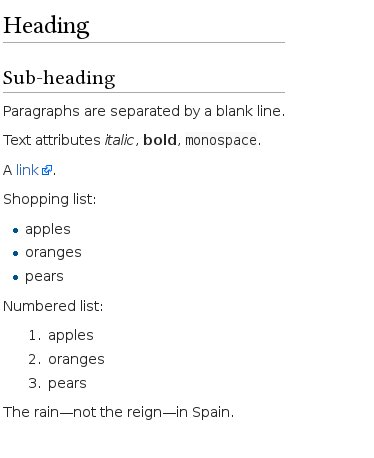
\includegraphics[width = .5\linewidth]{graphics/markdown.jpeg}
\end{frame}

\begin{frame}[fragile]
  \frametitle{knitr with Markdown} 
  Code chunk
  \begin{block}{}
\begin{verbatim}
```{r, echo=FALSE}
x <- rnorm(100)
```
\end{verbatim}
  \end{block}
\end{frame}

\end{document}
